\begin{frame}
    \frametitle{Příklad - JavaScript}
    \begin{figure}
        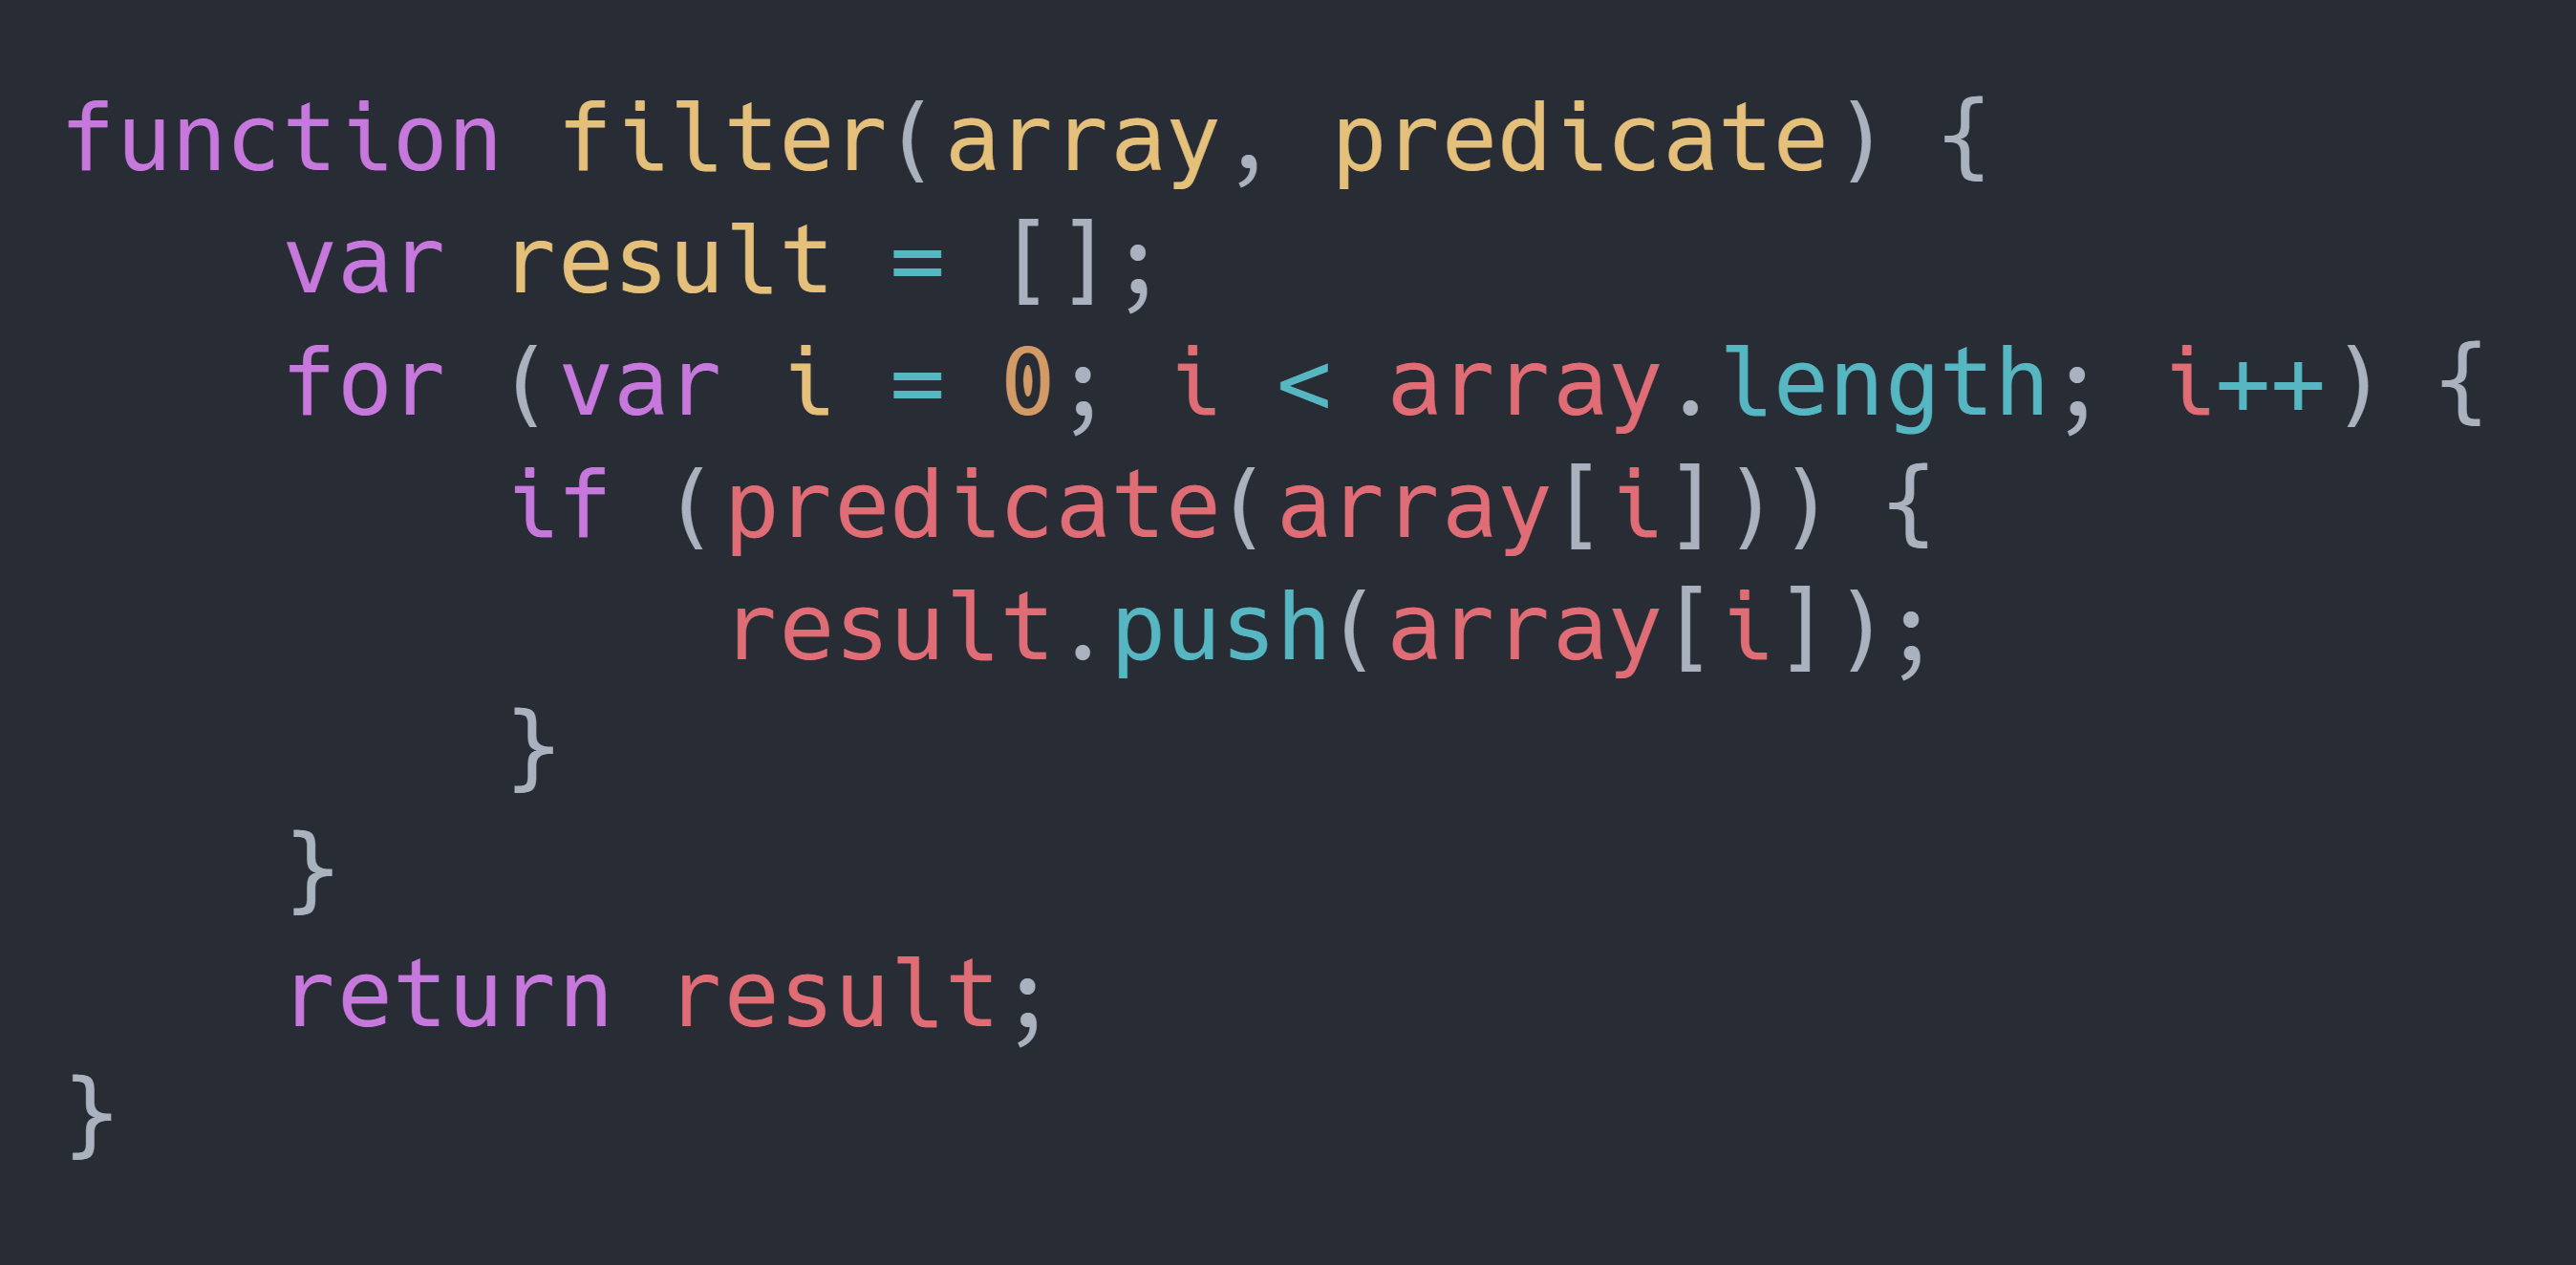
\includegraphics[width=300pt]{../resources/snippets/tsExample/example.js.png}
    \end{figure}
    
\end{frame}

\begin{frame}
    \frametitle{Příklad - TypeScript}
    \begin{figure}
        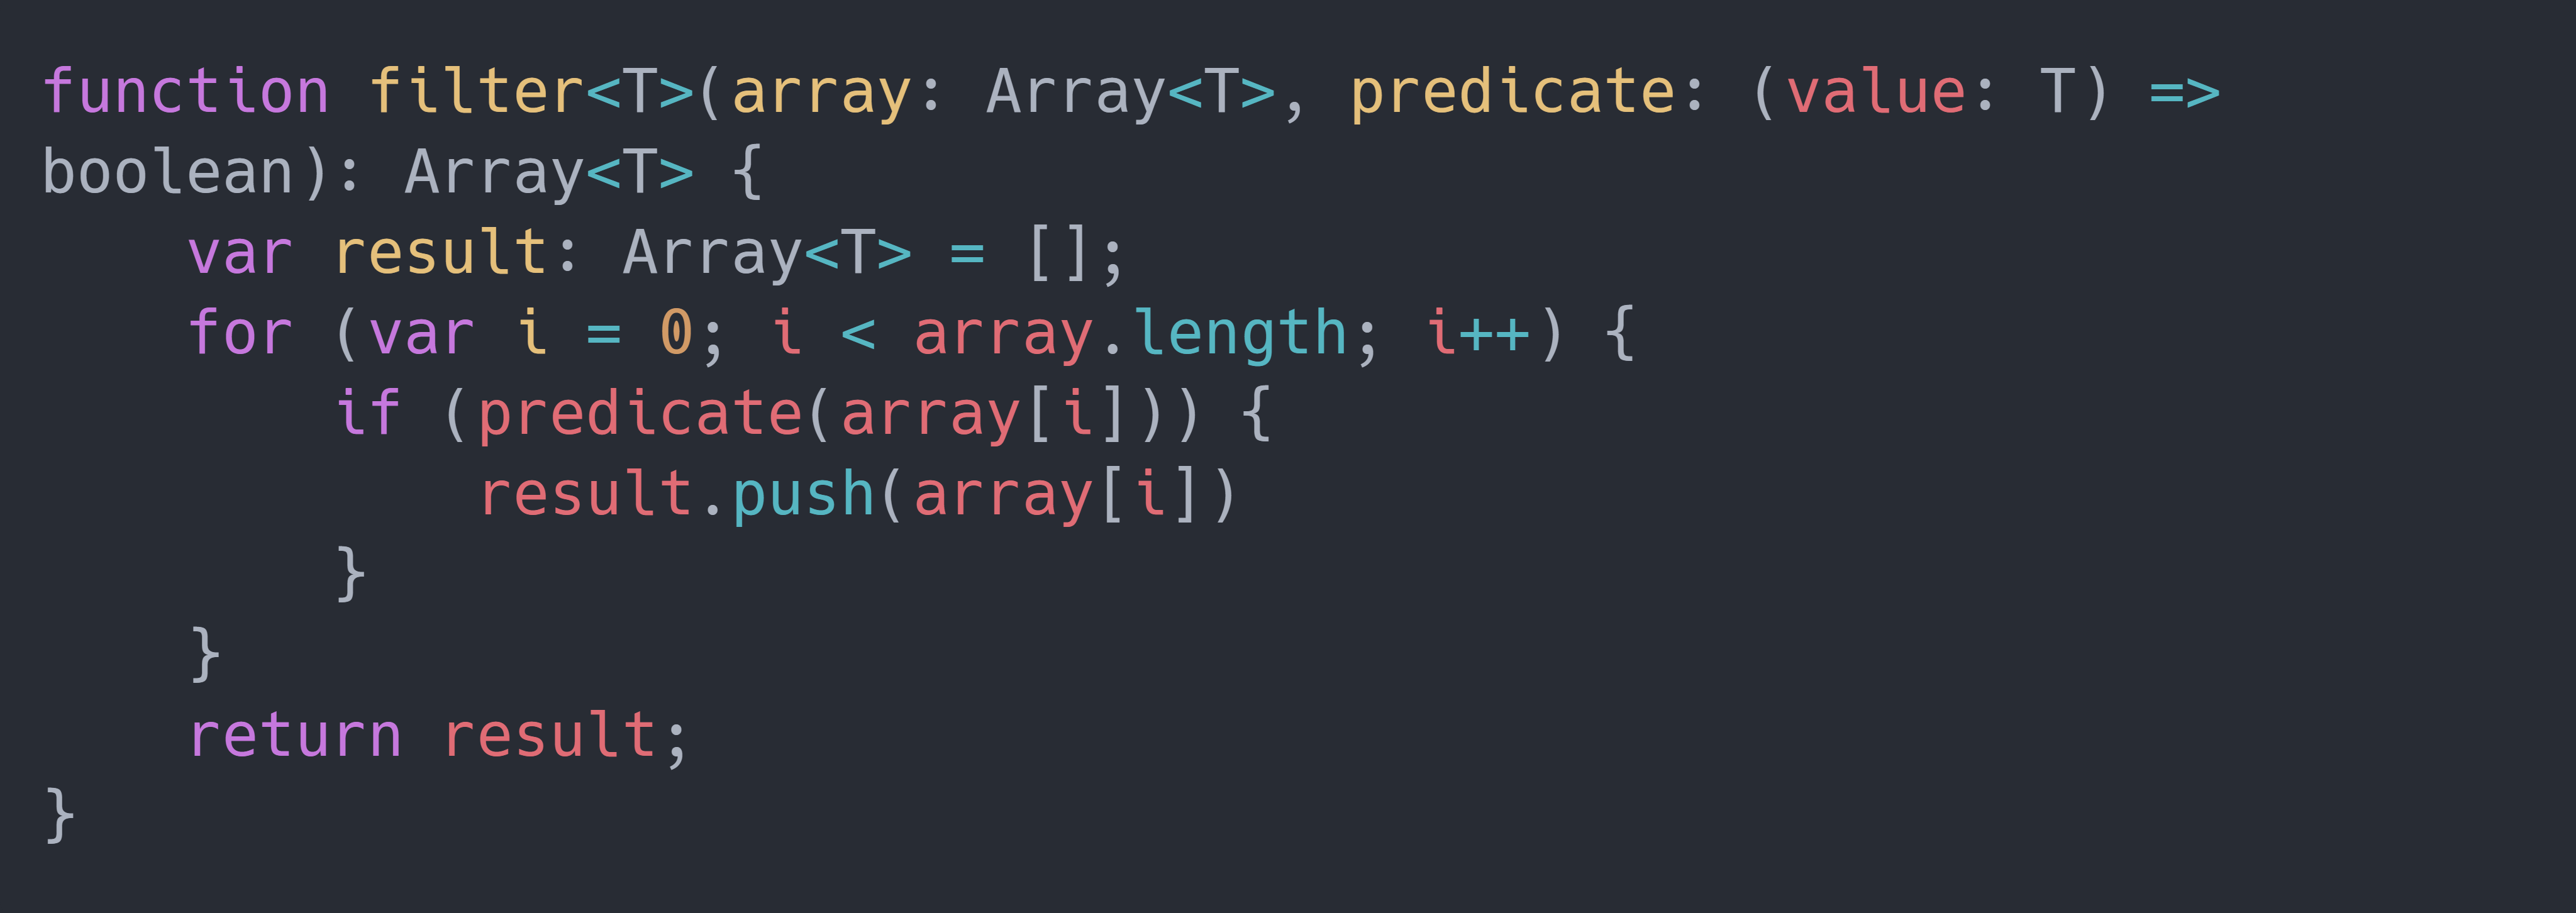
\includegraphics[width=300pt]{../resources/snippets/tsExample/example_rewritten.ts.png}
    \end{figure}
\end{frame}

\begin{frame}
    \frametitle{Příklad - TypeScript (moderní syntaxe)}
    \begin{figure}
        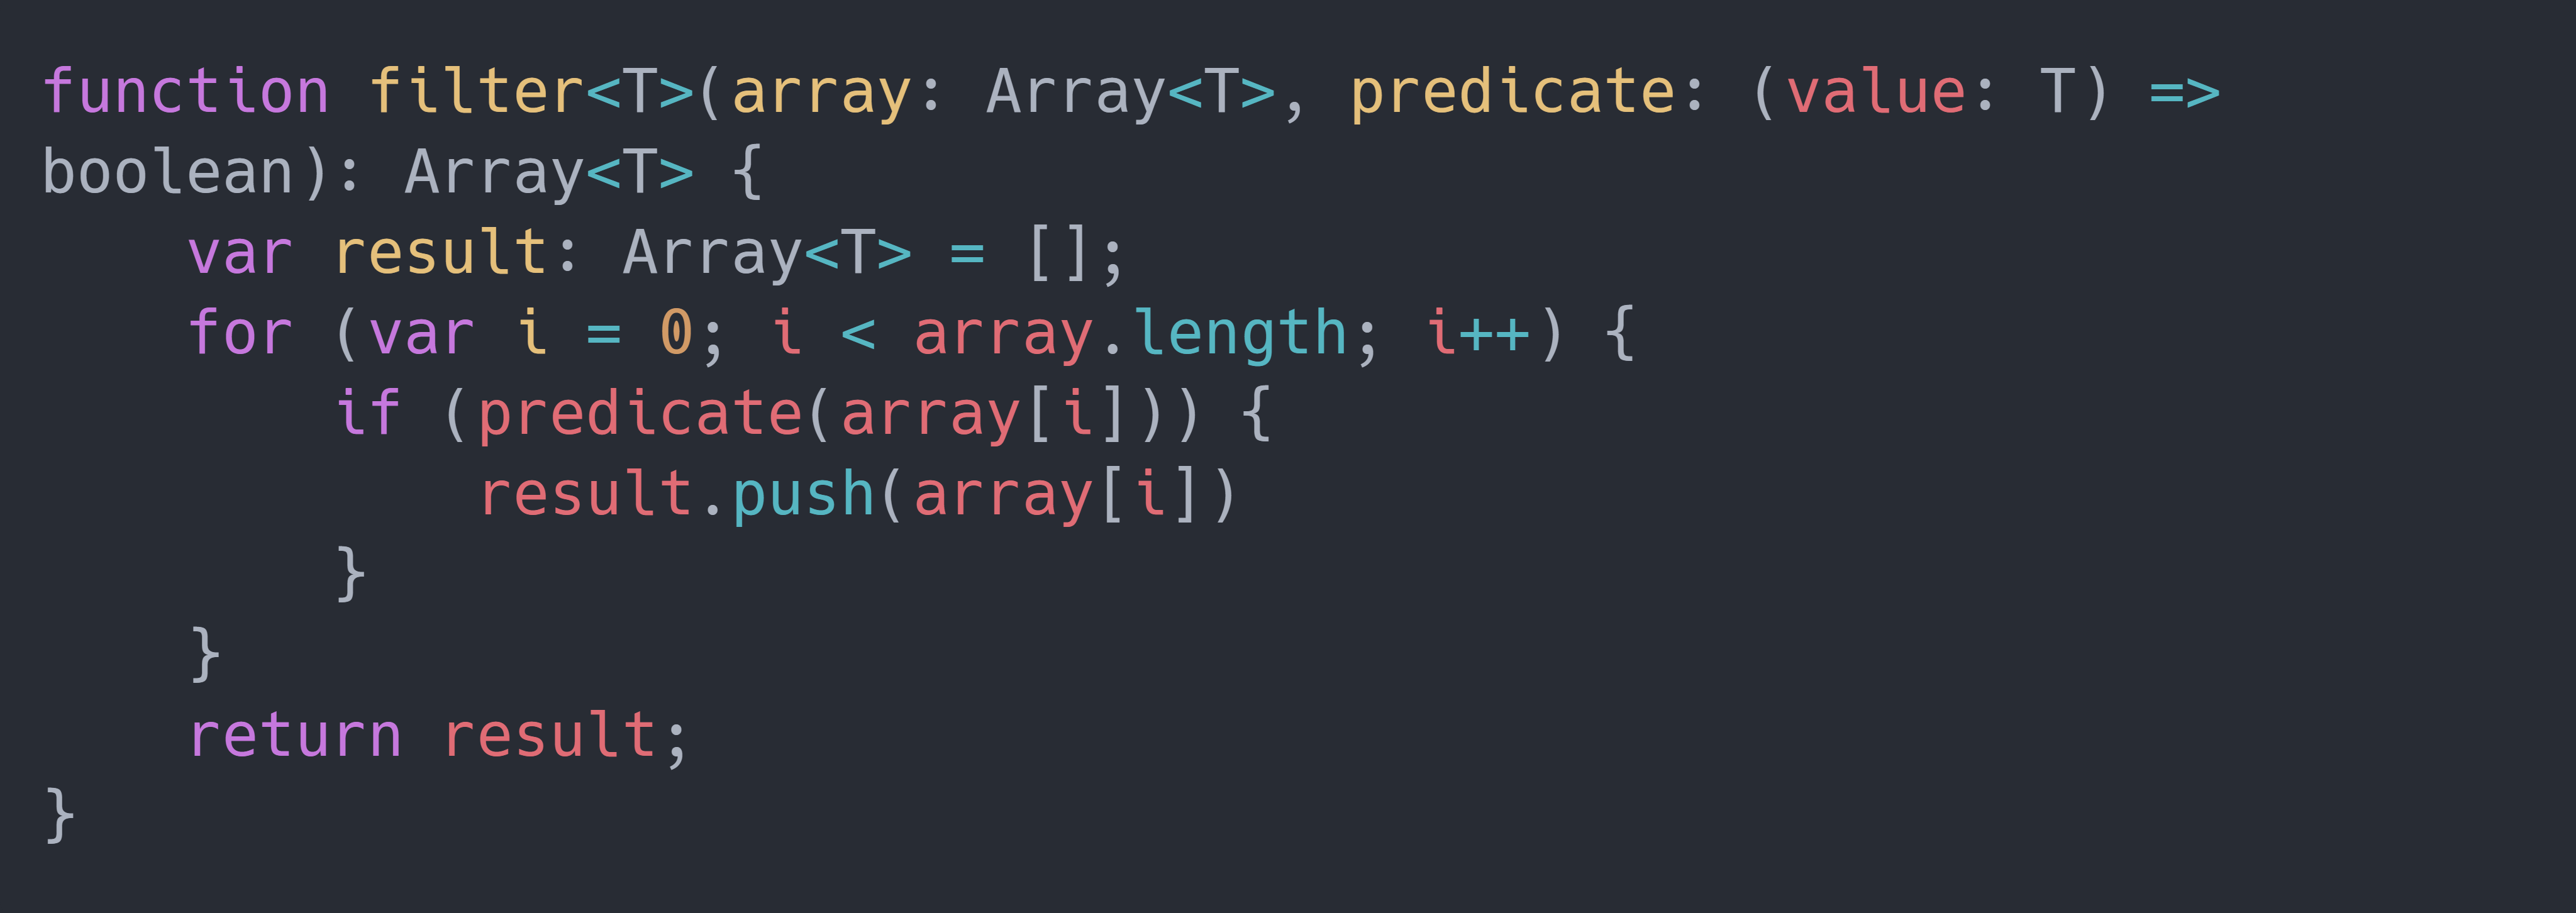
\includegraphics[width=300pt]{../resources/snippets/tsExample/example_rewritten.ts.png}
    \end{figure}
\end{frame}